\section{Introduction}
\label{sec:intro}
In this paper, we consider the current and future state of direct experimental searches for interactions of nuclei with dark matter masses approximately in the GeV to TeV range. This mass range, roughly corresponding to what has traditionally been labeled Weakly Interacting Massive Particle (WIMP) dark matter,  has historically received the most focus. Consequently, there is a broad competitive landscape of different targets and mature technologies. 
Complementary papers cover lighter~\cite{SnowmassCF1WP2} and heavier~\cite{SnowmassCF1WP8} direct detection searches as well as indirect searches via astronomical observation~\cite{SnowmassCF1WP5}. 

For the most part, sensitivity in this mass range does not depend strongly on experiment threshold. Rather, improvements in sensitivity are driven primarily by increasing exposure (i.e., target mass) and/or reducing backgrounds. Even for mature technologies that have already fielded multiple generations of detectors, scaling up the detector size presents numerous technical challenges. The most significant shared challenge is that backgrounds passing all fiducial and analysis cuts, both from radioactivity and instrument noise, must decrease proportionally with detector mass. Similarly calibration of detector response functions must improve with every successive generation. More details of these common concerns are presented in \cite{SnowmassCF1WP3}. Other challenges are unique to a given detector technology, such as affordably maintaining high signal collection efficiency while covering a larger area, further from the fiducial volume. To ensure success in further searches, R\&D investments both addressing how to scale up existing technologies as well as examining totally new technologies are warranted. 

If not limited by other factors, dark matter detectors will be limited by irreducible backgrounds from neutrinos~\cite{monroe2007, strigari2009, billard2014b}. Originally dubbed the ``neutrino floor,''  the community now promotes the term ``neutrino fog,'' to better indicate that, rather than a hard limit on direct detection sensitivity, the neutrino background imposes a gradual penalty that can be overcome, at least to some extent. In Section~\ref{sec:neutrinofloor} we quantify the effect of neutrino backgrounds on detector sensitivity versus exposure. 

In Section~\ref{sec:theory} we provide a survey of theoretically-motivated dark matter candidates in this mass range consistent with experimental evidence from dark matter searches, collider experiments, and astronomical observatories. As we shall show, this mass range is well-covered by predictive theories, down to and well into the neutrino fog. Very few of these theories will be fully tested by the upcoming generation of funded experiments. As described in Section~\ref{sec:currentexperiments}, the \textit{subsequent} generation of current experiments (``generation 3'') is expected to reach deep enough into the neutrino fog to incur significant diminishing returns on further growth.  Further exploration of this theoretically-motivated parameter space will require either extreme scaling of detector size or developing new technology less sensitive to neutrino backgrounds, as discussed in Section~\ref{sec:beyondnufog}.

Figure~\ref{fig:limitplot_SI} summarizes the current state of spin-independent dark matter cross section limits as well as the projected sensitivity of future experiments. For technologies so far in use or planned for the near future, the spin-dependent case is dominated by xenon for dark matter-neutron interactions and fluorine for dark matter-proton interactions. Fluorine additionally is several orders of magnitude less sensitive to coherent neutrino interactions than xenon and thus can reach significantly lower spin-dependent cross sections. 

\begin{figure}
    \centering
    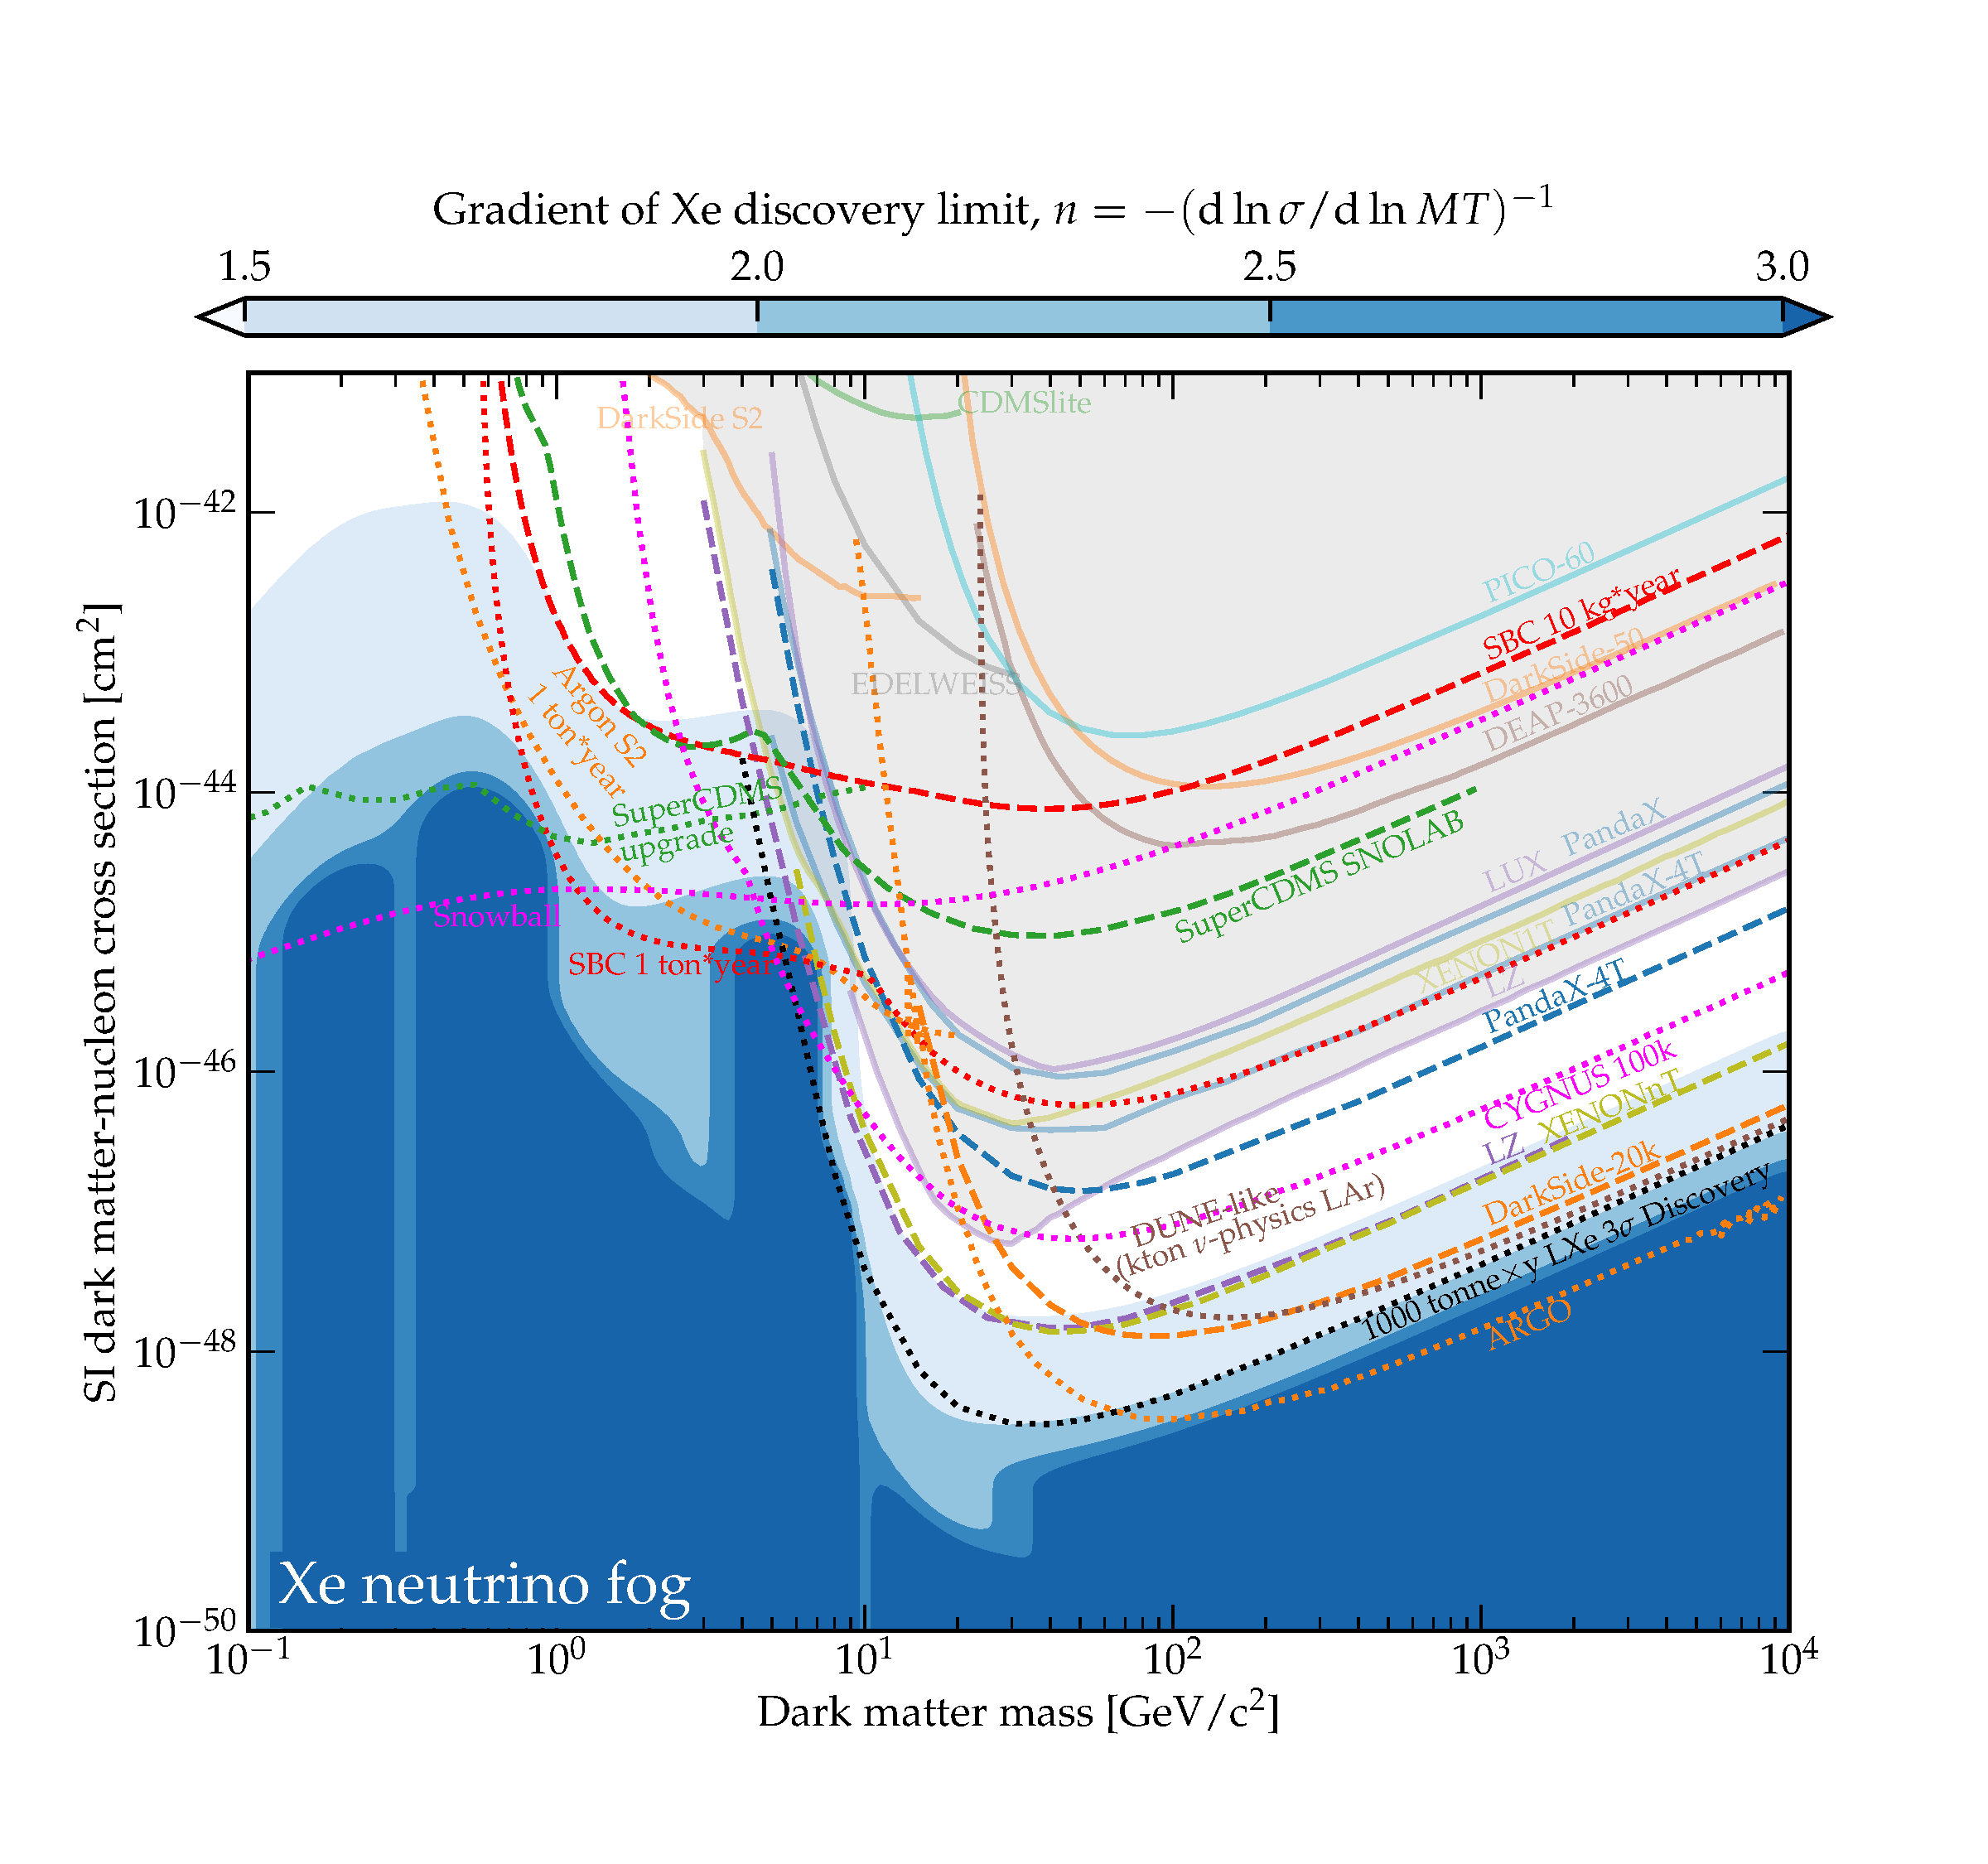
\includegraphics[width=\textwidth]{figures/CombinedLimitPlot_SI.pdf}
    \caption{Combined Spin-independent dark-matter nucleon scattering cross section space. Currently-excluded space is shaded gray~\cite{pandax-iicollaboration2017, picocollaboration2017, darksidecollaboration2018a, cresstcollaboration2019,hehn2016a,darksidecollaboration2018,luxcollaboration2017,xenoncollaboration2021,deapcollaboration2019,supercdmscollaboration2019a} (data points taken from~\cite{OHare:2021utq}). Dashed lines represent projected 90\% confidence level exclusion sensitivity of new experiments. Because not all experiments used the same methodology in estimating limits (e.g., single-sided upper likelihood vs two-sided), exact sensitivities may not be directly comparable. The neutrino fog for a xenon target is presented in the blue contour map as described in Section~\ref{sec:neutrinofloor}. At contour $n$, obtaining a 10$\times$ lower cross section sensitivity requires an increase in exposure of at least $10^n$. The $n=2$ fog contour for argon is also shown in the black wide-dashed line. LZ: 15 ton-year, one-sided upper limit. XENONnT: 20 ton-year with two-sided interval. PandaX-4T: 5.6 ton-year. DarkSide-20K: 200 ton-year. SuperCDMS: combined result of detector types; SuperCDMS upgrade refers to scenario C in Ref.~\cite{SuperCDMS_SNOWMASS22}. 
    \label{fig:limitplot_SI}}
\end{figure}
